\documentclass{article}
\usepackage{graphicx}

\title{An example of hybridising mosquito evolution in Africa}
\author{Andy Wilkins}

  
\begin{document}
\maketitle

\section{Introduction}

I describe a simple simulation using ODE dynamics defined by Beeton et al.\footnote{Beeton, Hosack, Wilkins, Forbes, Ickowicz and Hayes, Journal of Theoretical Biology 2019}, mainly as an example of the type of simulation that the code can perform.

\section{Cell dynamics}

The {\tt CellDynamicsBeeton2\_2} class is used.  This solves the coupled equations
\begin{eqnarray}
  \frac{{\mathrm d}X}{{\mathrm d}t} & = & \left[-\mu_{X} + \left(1 - \frac{X + \alpha_{XY}Y}{K_{X}}\right)\frac{X}{X + wY}\gamma_{X}\right] X \ , \\
  \frac{{\mathrm d}Y}{{\mathrm d}t} & = & \left[-\mu_{Y} + \left(1 - \frac{\alpha_{YX}X + Y}{K_{Y}}\right)\left( \gamma_{Y} + \frac{wX}{X + wY}\gamma_{X}\right) \right] Y \ ,
\end{eqnarray}
for populations $X(t)$ and $Y(t)$.  Beeton et al. describe various parameter scenarios, and here we explore the choice given in their Figure5(c).  That is:
\begin{itemize}
\item $\mu_{X} = 0.7$\,day$^{-1}$;
\item $\mu_{Y} = 0.8$\,day$^{-1}$;
\item $\gamma_{X} = 1.0$\,day$^{-1}$;
\item $\gamma_{Y} = 1.0$\,day$^{-1}$;
\item $\alpha_{XY} = \alpha_{YX} = 0.4$;
\item $w=0.05$.
\end{itemize}
The carrying capacities, $K_{X}$ and $K_{Y}$ vary spatially and temporally, as described below.

In the spatially-dependent simulations, both $X$ and $Y$ are assumed to diffuse and advect.  The ODE is solved for only occurs for 0.5 days out of each day.

\section{Simulation of the ODE only}
\label{sec.ode.only}

Beeton et al. describe a time-varying scnario where the carrying capacity $K_{X}=K_{Y}$ oscillates between $1$ and $0.2$ in a stepwise fashion, as in Figure~\ref{ode_K.fig}

\begin{figure}[htb]
  \centering
  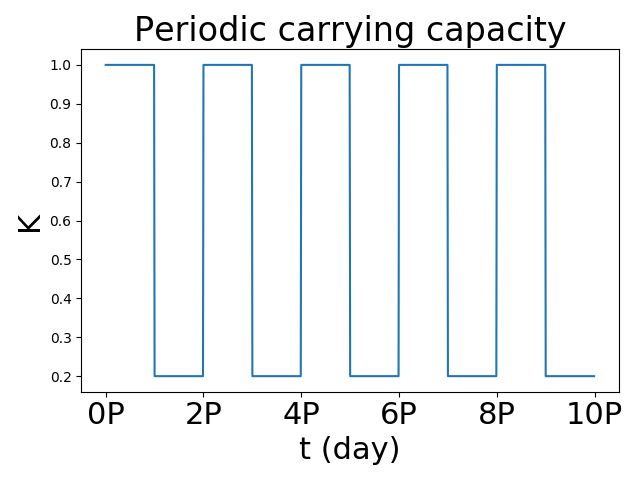
\includegraphics[width=5cm]{ode_K.png}
  \caption{\label{ode_K.fig}The periodic carrying capacity, depending on period $P$}
\end{figure}


They demonstrate that the evolution of $X$ and $Y$ can depend on the period of the oscillation.  This may be simulated using the current code (see the ``runner'' script {\tt ode\_only.py}) and results in Figure~\ref{ode_only.fig} that replicates Beeton et al.'s result

\begin{figure}[htb]
  \centering
  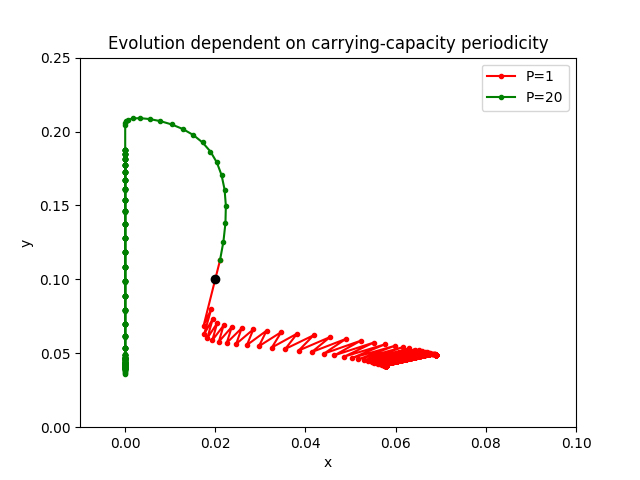
\includegraphics[width=6cm]{ode_only.png}
  \caption{\label{ode_only.fig}Replicating the scenario studied in Beeton et al., with oscillating carrying capacity.  The black dot shows the initial condition.  The dynamics depends on the periodicity, $P$ (measured in days) of the oscillation.  (Each dot in this diagram corresponds to the result after 1 day of simulation.)}
\end{figure}


\section{The spatial domain}

The spatial domain is defined by a $5$\,km$\times 5$\,km grid with lower-left corner at $(x,y)=(-4614,-3967)$ (km) and $n_{x}=1517$ and $n_{y}=1667$, that is
\begin{verbatim}
Grid(-4614.0, -3967.0, 5.0, 1517, 1667, False)
\end{verbatim}
The inactive cells are defined to be those in the ocean, while everything else is active.  This results in $1.4\times 10^{6}$ cells, as shown in Figure~\ref{active_inactive.fig}.

\begin{figure}[htb]
  \centering
  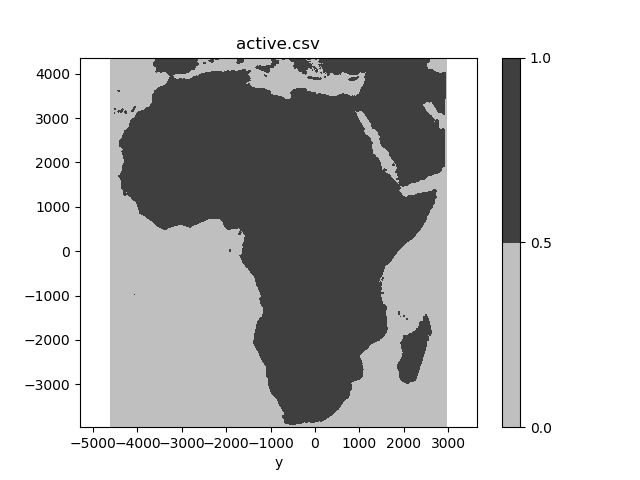
\includegraphics[width=9cm]{active.png}
  \caption{\label{active_inactive.fig}The spatial domain.  Active cells are dark-coloured.}
\end{figure}

\section{Carrying capacity}

Carrying capacity is based on the spatially varying function
\begin{equation}
  C(x,y) = \mbox{spatially-varying carrying capacity of Figure~\ref{carrying.fig}} \ .
\end{equation}
A time-dependent carrying capacity is used in some simulations, described below.

\begin{figure}[htb]
  \centering
  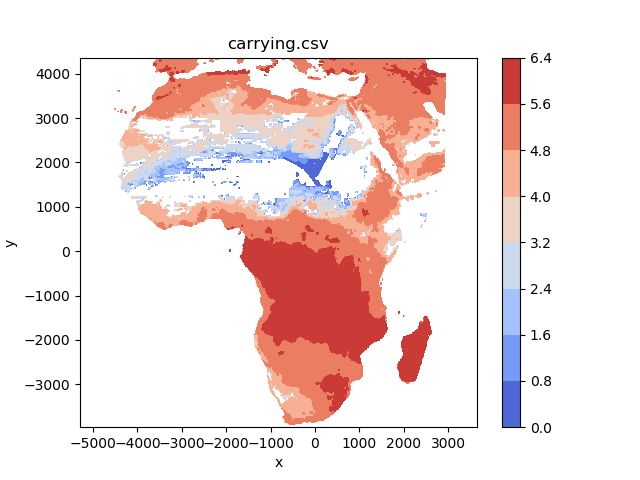
\includegraphics[width=9cm]{carrying.png}
  \caption{\label{carrying.fig}$\log_{10}C$ (mosquitoes per grid cell).}
\end{figure}

\section{Diffusion}

Diffusion is assumed to have a constant, uniform diffusion coefficient of $0.1$\,km$^{2}$.day$^{-1}$.

\section{Advection by wind}

Just one wind file is used, so wind is spatially-varying but temporally constant throughout the simulation.  It is assumed that 1\% of the population, $P$, of each cell enters the wind steam every day.

The probability distribution for mosquitoes to ``drop out'' of the wind stream is assumed to be exponential:
\begin{equation}
  p(t) \propto \left\{
  \begin{array}{ll}
    e^{-6t} & \ \ \mbox{for } t \leq 0.5 \\
    0 & \ \ \mbox{for } t > 0.5
  \end{array}
  \right.
\end{equation}
where $t$ is measured in days.  This gives $p(0)\approx 15$\% and $p(0.5) \approx 0.7$\%.  Hence, regardless of the time-step size, mosquitoes advect for up to 0.5 days every time step.

\section{Initial conditions}

It is assumed that initially
\begin{equation}
  Y(x, y, t=0) = C(x, y) \ ,
\end{equation}
and that $X(t=0)=0$, except for at cell $(x, y) = (-2000, 700)$, which is in the south of Nigera.  At this cell 10,000 mosquitoes are introduced.  This is shown in Figure~\ref{zoom_0.fig}.

\begin{figure}[htb]
  \centering
  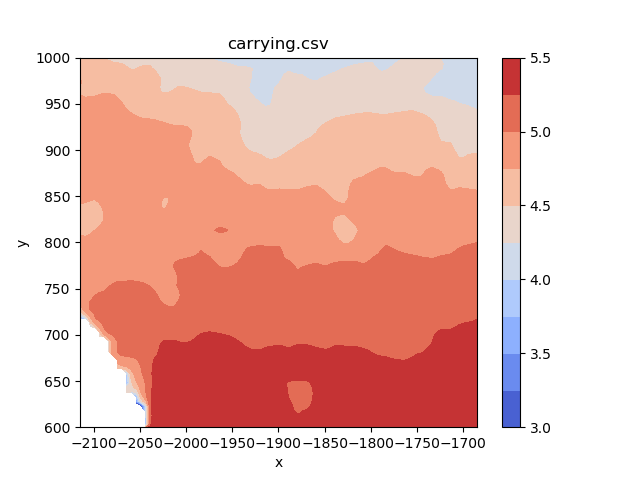
\includegraphics[width=5cm]{carrying_zoom.png} \quad
  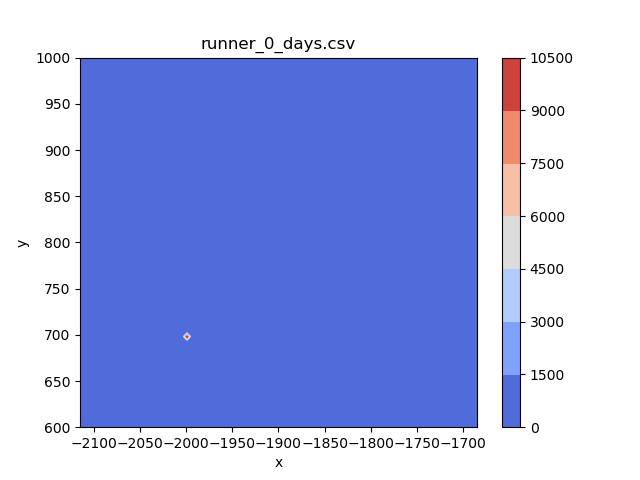
\includegraphics[width=5cm]{runner_0_days.png}
  \caption{\label{zoom_0.fig}Zoomed views into the region of interest.  Left: $\log_{10}C$.  Right: the initial population of X.}
\end{figure}

\section{Diffusion and advection only}

(Using {\tt runner.py})  When the ODE dynamics is not included in the simulation, the 10,000 ``X'' mosquitoes simply diffuse and advect.  The result after 200 days is shown in Figure~\ref{runner_x_no_cell_evolve_200_days.fig}

\begin{figure}[htb]
  \centering
  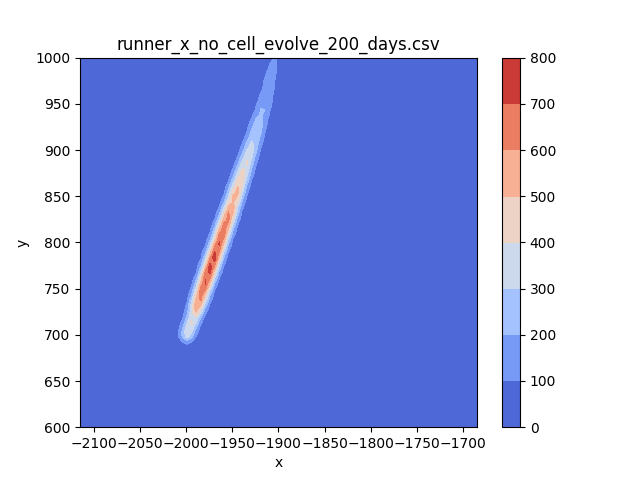
\includegraphics[width=7cm]{runner_x_no_cell_evolve_200_days.png}
  \caption{\label{runner_x_no_cell_evolve_200_days.fig}The population of ``X'' after 200 days of diffusion and advection without any ODE dynamics.}
\end{figure}


\section{Invasion of $X$}

(Using {\tt runner.py})  When
\begin{equation}
  K_{X} = C \ \mbox{ and }\ K_{Y} = C/5 \ ,
\end{equation}
the ODE dynamics evolves towards an $X$-dominant steady state.  Coupling this with advection and diffusion, the results after 200 days is shown in Figure~\ref{runner_x_highcc_200_days.fig}.

\begin{figure}[htb]
  \centering
  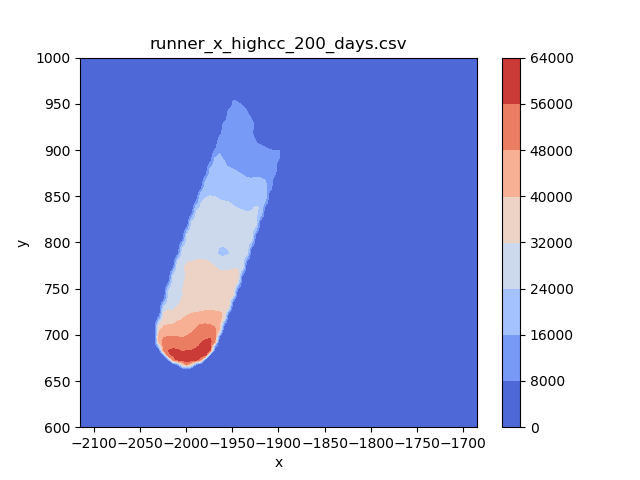
\includegraphics[width=5cm]{runner_x_highcc_200_days.png} \quad
  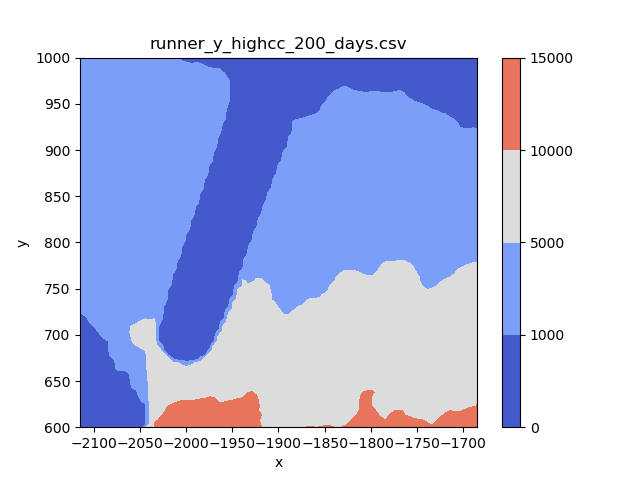
\includegraphics[width=5cm]{runner_y_highcc_200_days.png}
  \caption{\label{runner_x_highcc_200_days.fig}The population of $X$ (left) and $Y$ (right) after 200 days of evolution, diffusion and advection when the carrying capacity of $X$ is five times that of $Y$.}
\end{figure}


\section{Time-varying carrying capacities}

(Using {\tt runner.py})  Here I study a spatially-varying analogue of Section~\ref{sec.ode.only}.  That is
\begin{equation}
  K_{X} = K_{Y} = \beta(t) C(x, y) \ .
\end{equation}
where $\beta(t)$ oscillates between 1 and 0.2 in a stepwise fashion with periodicity $P$ (days): see Figure~\ref{ode_K.fig}.  The results after 200 days is shown in Figure~\ref{runner_x_P_1_200_days.fig}.

Although the ODE dynamics of shown in Figure~\ref{ode_only.fig} suggests there might be a difference between $P=1$\,day and $P=20$\,days, there is very little difference, and $X=0$ in cells neighbouring the release site.  What happens is that any $X$ that spreads to neighbouring cells gets immediately out-competed by the $Y$ that is present there.

\begin{figure}[htb]
  \centering
  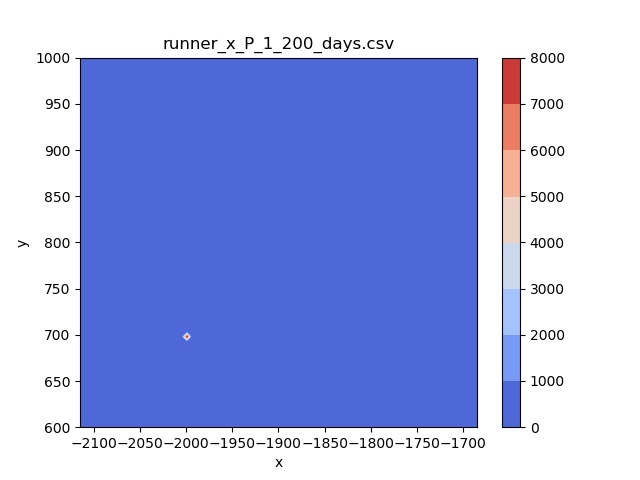
\includegraphics[width=5cm]{runner_x_P_1_200_days.png} \quad
  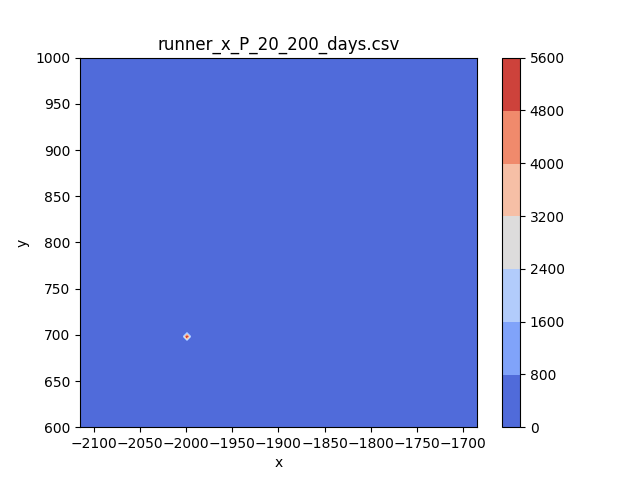
\includegraphics[width=5cm]{runner_x_P_20_200_days.png}
  \caption{\label{runner_x_P_1_200_days.fig}The population of $X$ after 200 days of evolution, diffusion and advection, when the carrying capacity oscillates between $C$ and $0.2C$ with periodicity $P$.  Left: $P=1$\,days.  Right: $P=20$\,days.}
\end{figure}


\section{Time-varying $K_{X}$}

(Using {\tt runner.py})  Here I study a spatially-varying analogue of Section~\ref{sec.ode.only}.  That is
\begin{equation}
  K_{X} = \beta(t) C(x, y) \ \ \mbox{ and }\ \  K_{Y} = 0.2 C(x, y) \ .
\end{equation}
where $\beta(t)$ oscillates between 1 and 0.2 in a stepwise fashion with periodicity $P$ (days).  The results after 200 days is shown in Figure~\ref{runner_Kxvary_x_P_1_200_days.fig}.

Evidently, there is a difference between $P=1$\,day and $P=20$\,days.  Comparing with Figure~\ref{runner_x_highcc_200_days.fig} there is less lateral diffusion (perpendicular to the prevailing wind direction) as the $X$ that spreads laterally to neighbouring cells gets out-competed by the $Y$ that is present there.

\begin{figure}[htb]
  \centering
  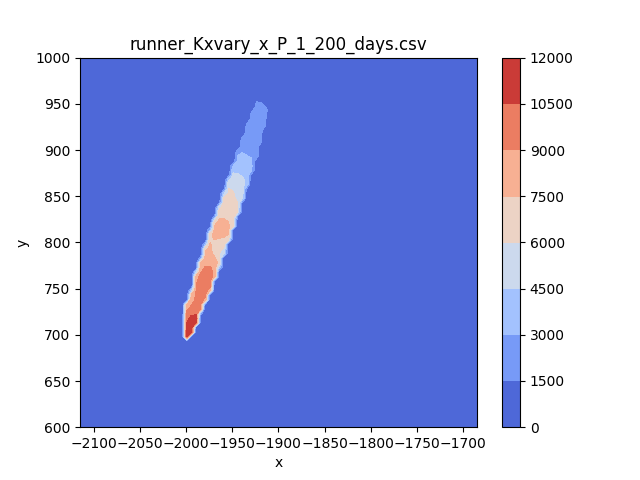
\includegraphics[width=5cm]{runner_Kxvary_x_P_1_200_days.png} \quad
  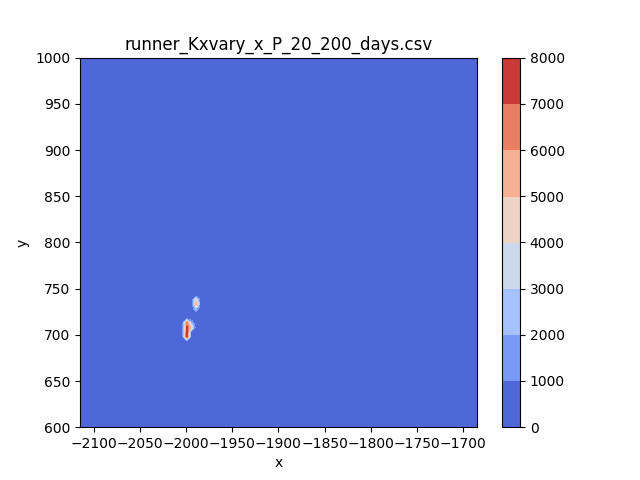
\includegraphics[width=5cm]{runner_Kxvary_x_P_20_200_days.png}
  \caption{\label{runner_Kxvary_x_P_1_200_days.fig}The population of $X$ after 200 days of evolution, diffusion and advection, when the carrying capacity $K_{X}$ oscillates between $C$ and $0.2C$ with periodicity $P$, and $K_{Y}=0.2C$.  Left: $P=1$\,days.  Right: $P=20$\,days.}
\end{figure}

\end{document}
